\chapter{Progettazione Concettuale/Logica}
Sebbene i database \emph{NoSQL} vengano definiti \emph{schemaless}, la progettazione dell'organizzazione dei dati richiede
di prendere decisioni significative. Infatti, i dati persistenti delle applicazioni hanno un impatto sui principali requisiti
di qualitá che devono essere soddisfatti in un'applicazione vera e propria (scalabilitá, prestazioni, coerenza).
Il mondo NoSQL é altamente eterogeneo, quindi questa attivitá di progettazione di solito si basa su pratiche e linee guida da seguire
in base al sistema adoperato. Peró, sono stati studiati diversi approcci che vogliono generalizzare il problema di progettazione
che é alla base di ogni sistema di persistenza.

\emph{NoAM} é uno dei principali strumenti di modellazione astratto per database NoSQL. Grazie ad esso riusciamo a definire
una progettazione che é indipendente dal sistema specifico in cui viene usata. Viene utilizzato un modello dei dati intermedio e astratto,
che, a sua volta, viene utilizzato per rappresentare i dati dell'applicazione come raccolte di oggetti aggregati.
\section{Modellazione NoAM $\to$ NoSQL abstract model}
La metodologia \emph{NoAM} é composta da:
\begin{itemize}
    \item Modellazione Concettuale e design degli Aggregati
    \item Partizionamento degli Aggregati e modellazione NoSQL
    \item Implementazione
\end{itemize}

\subsection{Modellazione Concettuale e design degli Aggregati}
Riguarda la vera e propria progettazione del modello di dominio, e comporta l'identificazione
delle diverse classi di aggregati necessari in un'applicazione.

\paragraph{Cos'é un aggregato?}
Un aggregato é una porzione di dati correlati, con una struttura piú o meno complessa ed ha un identificatore univoco.
Gli aggregati regolano anche la distribuzione dei dati, infatti per supportare la scalabilitá sono distribuiti tra i nodi
di un sistema;
ogni oggetto aggregato si trova su un singolo nodo.\\

Sono possibili diversi approcci per identificare classi di aggregati per una particolare applicazione.
L'approccio Domain-Driven Design(\emph{DDD}), attraverso il quale viene generato un diagramma UML delle classi,
é guidato dai casi d'uso, ovvero dai requisiti funzionali, e da esigenze di scalabilitá e coerenza all'interno dell'aggregato.\\
Si procede nel modo seguente:
\begin{itemize}
    \item I dati persistenti di un'applicazione sono modellati in termini di entitá, oggetti di valore e
    relazioni.
    Un'entitá é un oggetto persistente che ha un'esistenza indipendente ed é caratterizzata da un identificatore
    univoco, mentre un oggetto di valore é caratterizzato appunto da un suo valore senza un proprio identificatore
    \item Entitá e oggetti di valore vengono raggruppati in \emph{aggregati}.
    Un aggregato ha un'entitá come radice e puó contenere molti oggetti di valore.
\end{itemize}
A causa delle loro caratteristiche, la progettazione degli aggregati comporta un compromesso per quanto riguarda
la loro granularitá.
Infatti:
\begin{itemize}
    \item Gli aggregati dovrebbero essere abbastanza grandi per poter includere tutti i dati coinvolti da
    certi vincoli di integritá.
    \item Gli aggregati dovrebbero essere i piú piccoli possibile, in quanto dimensioni ridotte consentono di
    soddisfare requisiti di prestazioni e scalabilitá.
\end{itemize}
Preso come esempio un dominio in cui vanno salvati in modo persistente dati su giocatori e giochi

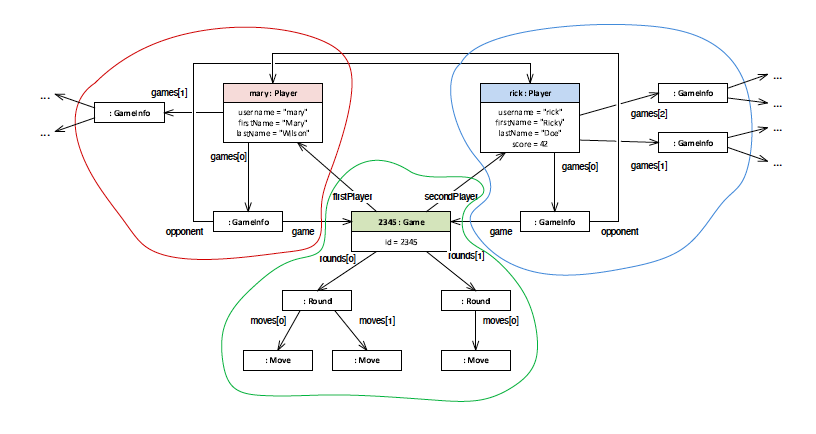
\includegraphics[width=1.05\textwidth]{img/designAggregati}
Nella figura sopra riportata l'oggetto con lo scomparto superiore colorato é un'entitá, altrimenti
é un oggetto di valore. La linea chiusa denota il confine di un aggregato.
Pertanto avremo due classi aggregate principali: Player e Game.\\
Quindi, per costruire un'aggregato si parte sempre da un'entitá principale.
Le freccie uscenti indicano la composizione dell'entitá e, ricorsivamente, degli oggetti di valore.
Se consideriamo l'entitá \texttt{mary:Player}, essa sará composta, oltre che dai suoi attributi, da:\\
due oggetti di valore, rispettivamente \texttt{games[0]} e \texttt{games[1]}, a sua volta \texttt{games[0]} é formato dall'oggetto
di valore \texttt{:GameInfo} cosí composto:\\
il valore di \texttt{game} sará \texttt{2345:Game}, il valore di \texttt{opponent} sará composto da \texttt{rick:Player}.
Stesso procedimento verrá fatto per \texttt{games[1]}.\\
Bisognerá ripetere il procedimento per ogni entitá presente nel diagramma.


\subsection{Partizionamento degli Aggregati e modellazione NoSQL}
In questa fase viene utilizzato \emph{NoAM} come modello intermedio tra gli aggregati e i database NoSQL, quindi potrebbe
essere visto come un equivalente della \emph{progettazione concettuale} fatta nei database relazionali.
Il modello NoAM $\to$ modello di dati astratti, ha il compito di sfruttare i punti in comune dei vari modelli di dati, ma
introduce anche astrazioni per bilanciare le variazioni che vi sono tra diversi modelli di NoSQL.\\
Da questa trasformazione si ottengono due strutture con diverse granularitá:\\
\begin{itemize}
    \item \texttt{blocco}, unitá di dimensione maggiore, ha massima consistenza
    \item \texttt{entry}, unitá di dimensione minore, che permette l'accesso ai dati
\end{itemize}
Con riferimento in particolare ai database chiave-valore una \texttt{entry} corrisponde a una coppia chiave-valore, mentre
un \texttt{blocco} corrisponde a un gruppo di coppie chiave-valore correlate tra loro.

Quindi, si ha che:\\
Un \texttt{database} é un insieme di \texttt{collections};\\
Ogni \texttt{collection} ha un nome distinto; Una \texttt{collection} é un insieme di \texttt{blocchi};\\
Ogni \texttt{blocco} all'interno della \texttt{collection} é identificato da una chiave di blocco, che deve essere univoca;
Un \texttt{blocco} é un insieme non vuoto di \texttt{entries};\\
Ogni \texttt{entry} é composta da una coppia chiave-valore, la quale é univoca all'interno del blocco, il valore puó essere anche complesso.

Per effettuare il passaggio da aggregati a modellazione NoSQL, ogni classe di aggregati viene rappresentata da una \texttt{collection} ed
ogni singolo aggregato viene rappresentato da un \texttt{blocco}.\\
Un paragone puó essere fatto con la programmazione ad oggetti, in cui una \texttt{collection} é
una classe, ed un \texttt{blocco} é l'istanza di quella classe.

Vi sono due modalitá principali per rappresentare gli aggregati:
\begin{itemize}
    \item \emph{Entry per Aggregate Object (EAO)}: Rappresenta ogni aggregato utilizzando una singola
    \texttt{entry}, la chiave della \texttt{entry} é vuota, il valore contiene l'intero aggregato.
    Metodologia dedicata maggiormente ai database documentali.
    \item \emph{Entry per Atomic Value (EAV)}: Rappresenta ogni aggregato per mezzo di piú \texttt{entry};
    Nella fase successiva, ovvero quella di implementazione, le chiavi di ogni \texttt{entry} verranno utilizzate
    insieme al nome della collection ed alla chiave di blocco per creare una chiave con un
    nome strutturato e rendere piú semplice la ricerca;
    i valori di ogni \texttt{entry} sono atomici.\\
    Questa metodologia é proprio quella che rispecchia in modo piú appropriato i database key-value.
\end{itemize}
\vspace{0.5cm}
    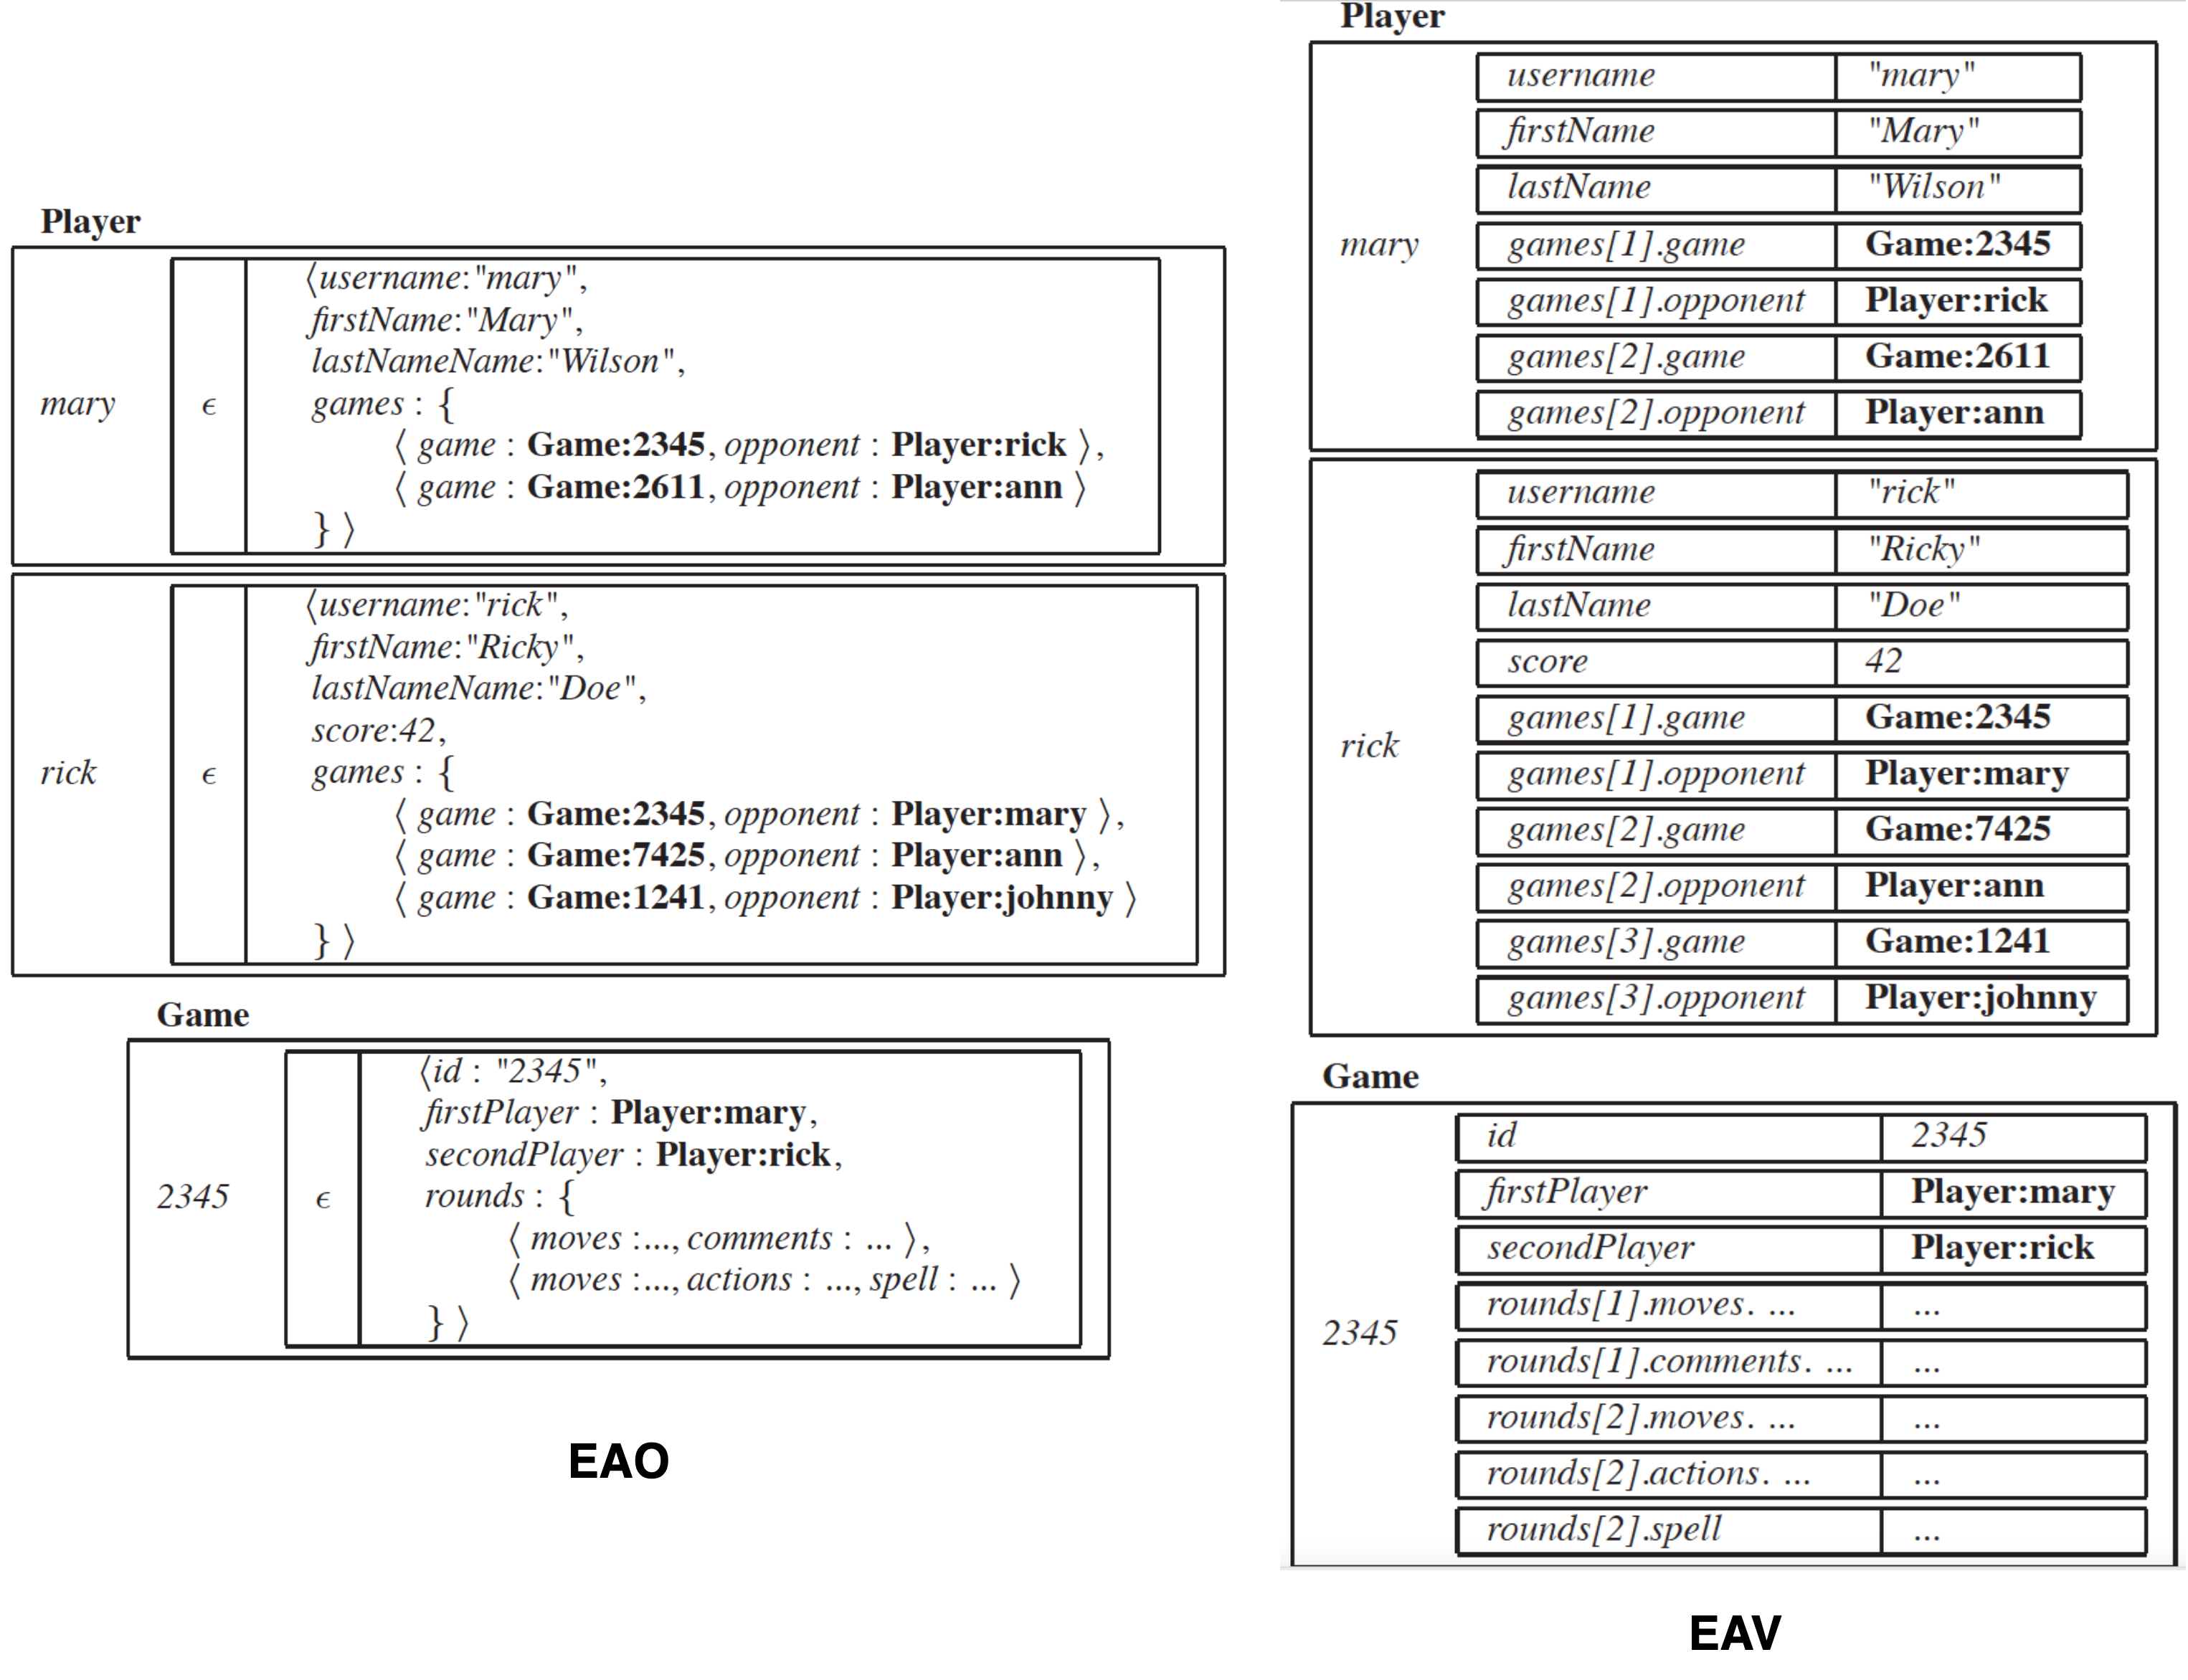
\includegraphics[width=1\textwidth]{img/eao.eav}
Nella figura \emph{EAO} si ha per ogni \texttt{blocco} \emph{Player} o \emph{Game} una singola \texttt{entry} con chiave vuota,
valore strutturato in modo complesso
\\
Nella figura \emph{EAV} si ha per ogni \texttt{blocco} piú \texttt{entry} in modo da avere valori atomici al suo interno
\\
\\
Ovviamente queste due sono le rappresentazioni piú estreme che si possono ottenere.
É possibile adottare una strategia di rappresentazione intermedia, denominata \emph{Entry per Top level Field (ETF)}, in cui
viene utilizzata una \texttt{entry} distinta per ogni campo di livello superiore, quindi si ha una sorta di struttura mista.
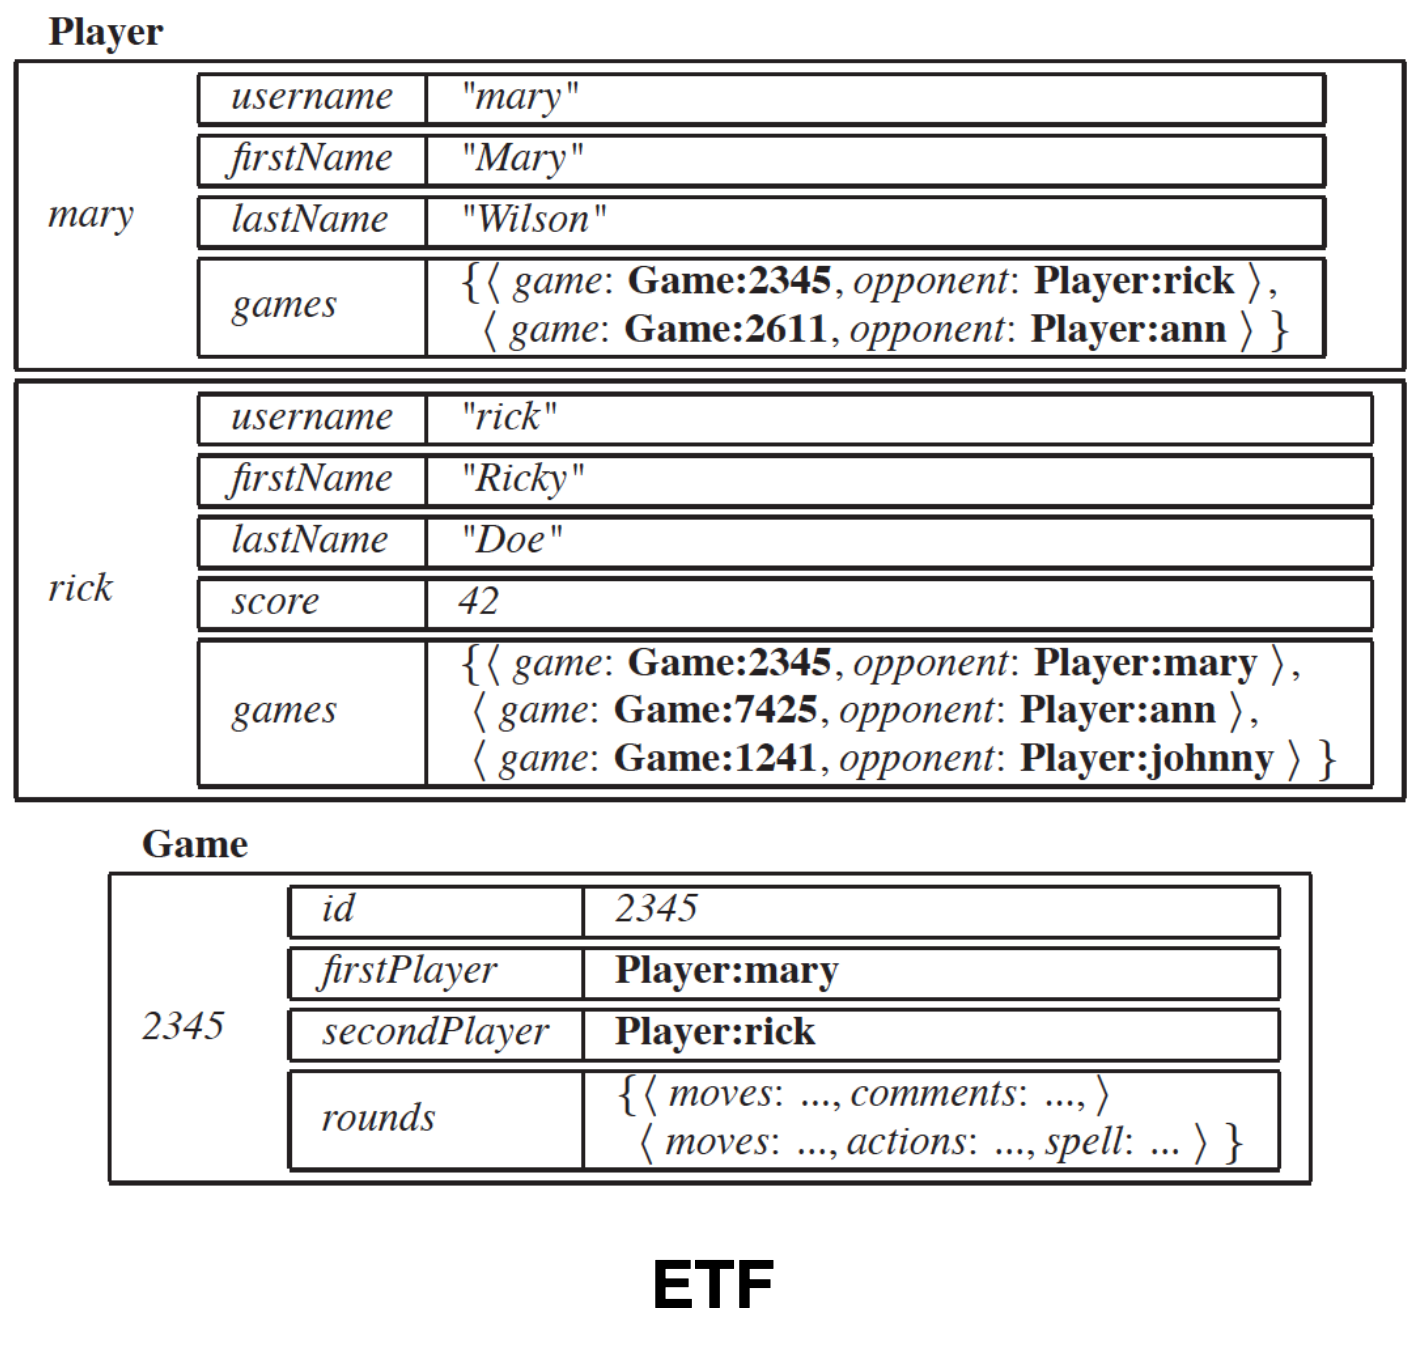
\includegraphics[width=0.8\textwidth]{img/etf}

Se dovessimo aver bisogno di una rappresentazione degli aggregati ancora piú flessibile é possibile effettuarne il \emph{partizionamento},
ovvero si possono raggruppare \texttt{entry} che vengono accedute insieme, oppure separare certe \texttt{entry} per avere dei
valori meno complessi.

\subsection{Implementazione}
Consiste nel tradurre i modelli NoAM ottenuti nella fase precedente in strutture corrette per il dbms specifico che stiamo utilizzando.
Per quanto riguarda i database chiave-valore si utilizzerá una coppia chiave-valore per ogni \texttt{entry} ottenuta nella struttura
precedente.\\
In base alle scelte di progetto si decide quale modello NoAM utilizzare (EAO/EAV/ETF); bisogna decidere che livello di
complessitá vogliamo avere su chiavi e valori.
Se vogliamo ottenere dei valori semplici, rappresentabili semplicemente con dei tipi atomici, utilizzeremo il metodo \emph{EAV}, questo, peró, comporterá una maggiore complessitá delle chiavi.
Mentre, se vogliamo chiavi molto semplici dovremo utilizzare \emph{EAO}, peró otterremo dei valori strutturati e complessi, quindi, dovremo anche confrontarci con
il dbms di cui disponiamo per verificare se saranno presenti delle strutture dati adatte a rappresentare dei valori con un certo livello di complessitá, cosa non sempre
presente nei database key-value.\\

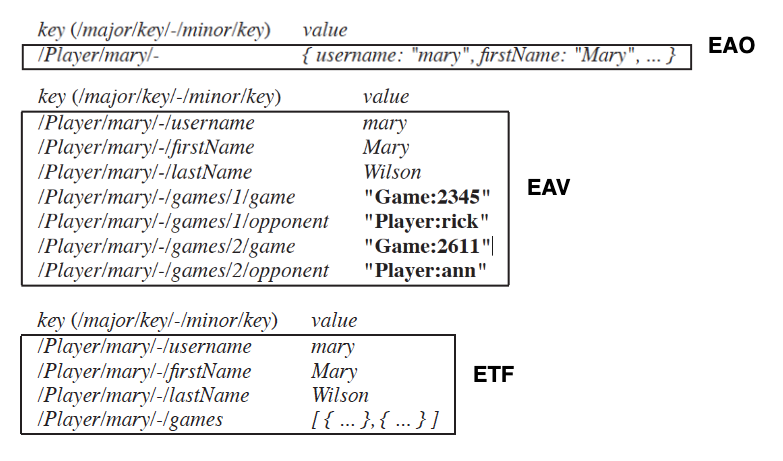
\includegraphics[width=1\textwidth]{img/implementazione}

La figura \emph{EAV} é quella che rispecchia maggiormente un database key-value classico con valori atomici.
Si puó notare che le chiavi hanno una struttura gerarchica, si ha una larga somiglianza con il directory service dei sistemi operativi;
questo viene fatto principalmente per facilitare la ricerca dei valori nelle interrogazioni.
%inserire immagine che mostra differenza tra progettazione relazione (foto che si puo prendere dalle slide di basi di dati) e
%creare schema a blocchi che rappresenta questa progettazione